\documentclass[10pt, a4paper, titlepage, fleqn]{article}

%packages
\usepackage[latin9]{inputenc}
\usepackage[ngerman]{babel}
\usepackage[T1]{fontenc}
\usepackage{amsmath}
\usepackage{amssymb}
\usepackage{graphicx}
\usepackage[a4paper,
left=3cm, right=1.5cm,
top=2.5cm, bottom=2.5cm]{geometry}

\usepackage{listings}
\lstset{language=Octave, basicstyle=\tt, tabsize=8,
  breaklines=true, caption=\texttt\lstname, captionpos=b}
\DeclareFontShape{OT1}{cmtt}{bx}{n}
{<5><6><7><8><9><10><10.95><12><14.4><17.28><20.74><24.88>cmttb10}{}

%\linespread{1.5}
\parindent 0pt

\pagestyle{headings}

\begin{document}

\begin{titlepage}
\title{3.Projekt f�r Numerische Mathematik UE \\
Numerische Quadratur}
\author{Thomas Baumhauer, Judith Braunsteiner,\\
Gabriel Ebner, Johannes Hafner,\\
Clemens M�llner, Christina Satzinger}
\date{\today}
\maketitle
\end{titlepage}

\section{Numerische Integration}

Anhand von 3 Verfahren soll ein Softwarepaket zur numerischen Integration bereitgestellt werden.\\

Wir haben hierf�r die folgenden Grundverfahren implementiert:

\begin{itemize}
\item Newton-Cotes-Integration
\item Romberg-Verfahren
\item Gauss-Legendre-Integration
\end{itemize}

Anschlie�end haben wir versucht, eine sinnvolle Anwendung auf Teilintervallen zu finden.

\subsection{Newton-Cotes-Formeln}

\subsubsection{Prinzip}

Die Newton-Cotes-Formeln verwenden eine Approximation des Integranden durch Lagrangepolynome.

F�r gegebene �quidistante St�tzstellen $x_0, \dots x_n$ gilt:

\begin{align*}
\int_a^b f(x) dx \approx \int_a^b p_n(x) dx = (b-a) \cdot \sum_{i = 0}^n w_i \cdot f(x_i)
\end{align*}

mit 

\begin{align*}
w_i = \frac{1}{b-a} \int_a^b \prod _{j = 0, i \neq j}^n \frac{x-x_j}{x_i-x_j} dx
\end{align*}.

Die Koeffizienten lassen sich nach Skriptum Seite 188 (MATLAB-Beispiel) auch �ber ein lineares Gleichungssystem bestimmen.
Aus Effizienzgr�nden berechnen wir alle benutzten Koeffizienten vor.

Wegen der speziellen Wahl der St�tzstellen integrieren die Quadraturformeln bei ungeradem n Polynome bis zum Grad n, bei geradem n sogar bis zum Grad n+1 exakt. Somit sind Quadraturformeln mit geradem n (also einer ungeraden Anzahl an St�tzstellen) denen mit ungeradem n vorzuziehen. Wir verwenden in unserer Implementierung deshalb nur die mit geradem Grad.

\subsubsection{Fehlerabsch�tzung}

Betrachtet man den Verfahrensfehler bei $x_i = a + i* \frac{b-a}{n}$, so erh�lt man
\begin{align*}
E(f) &= \left|\int_a^b f(x) dx - \int_a^b p_n(x) dx \right| \\
     &=\left| \int_a^b (f(x) - p_n(x)) dx \right| \\
     &= \left|\int_a^b - \frac{f^{(n+1)}(\zeta)}{(n+1)!} \cdot \prod_{j = 0}^n (x-x_j) dx \right| \\
     &= \left|\frac{f^{(n+1)}(\zeta)}{(n+1)!} \int_a^b \prod_{j = 0}^n (x - a - i \cdot \frac{b-a}{n}) dx \right| \\
     &\leq \left| f^{(n+1)}\right|_{\infty} \cdot K
\end{align*}.

mit 
\begin{align*}
K = \frac{1}{(n+1)!} \cdot \left| \int_a^b \prod_{j = 0}^n (x - (a + i \cdot \frac{b-a}{n})) dx \right| 
\end{align*}

Diese a priori Absch�tzung ist zur Laufzeit jedoch leider eher unbrauchbar. Wir verwenden stattdessen die relative �nderung des Ergebnisses. Ist diese zu klein, so wird abgebrochen.

\begin{align*}
F = \frac{p(n) - p(n-1)}{p(n)}
\end{align*}

\subsubsection{Implementierung}

Die Berechnung der Koeffizienten erfolgt nach:

\lstinputlisting{newton_cotes_weights.m}
 
Unsere Implementierung der Newton-Cotes-Quadratur sieht dann folgenderma�en aus:
 
\lstinputlisting{newton_cotes.m}

\subsection{Romberg-Quadratur}

\subsubsection{Prinzip}

Bei der Romberg-Quadratur wird von der summierten Trapezregel ausgegangen.
Wir w�hlen Schrittweite $h_n = \frac{b-a}{2^{n-1}}$

\begin{align*}
\int_a^b f(x) dx = \lim_{k \rightarrow \infty} I_{1,k}
\end{align*}

wobei 

\begin{align*}
I_{1,1} &= \frac{b-a}{2^n} \dot (f(b) + f(a))\\
I_{n,1} &= \frac{b-a}{2^n} \cdot \left( f(a) + f(b) + 2 \cdot \sum_{i = 1}^{2^{n-1}-1} f(a + \frac{i \cdot (b-a)}{2^{n-1}} \right)\\
I_{n,k} &= I_{n+1, k-1} + \dfrac{I_{n+1, k-1} - I_{n, k-1}}{2^{2 \cdot (k-1)}-1}
\end{align*}.

Das Schema kann also rekursiv nach dem Nevilleverfahren, welches wir in der speichersparenden Version (nur die Diagonale wird gespeichert) implementiert haben, berechnet werden.

\subsubsection{Fehlerabsch�tzung}

Will man den Fehler absch�tzen, so erh�lt man man a priori eine Fehlerabsch�tzung, die von gewissen Ableitungsschranken abh�ngt. 

Da dies zur Programmlaufzeit nicht sinnvoll zu bestimmen ist, wurde hier ebenfalls die relative �nderung des berechneten Wertes bestimmt.

\begin{align*}
F = \frac{I_{1, n} - I_{1, n-1}}{I_{1,n}}
\end{align*}

\subsubsection{Implementierung}

Unser Quellcode sieht folgenderma�en aus:

\lstinputlisting{romberg.m}

\subsection{Gau�-Quadratur}

\subsubsection{Prinzip}

Hier werden die Gewichte und St�tzstellen so gew�hlt, dass die Approximation optimal ist.

\begin{align*}
\int_a^b f(x) dx \approx \int_a^b g dx = (b-a) \cdot \sum_{i = 0}^n w_i \cdot f(x_i)
\end{align*}

Nach Satz 6.5 gilt folgendes:

\begin{itemize}
\item Die Gewichte $w_i$ erf�llen 
\begin{align*}
w_i = \int_a^b \prod _{j = 0, i \neq j}^n \frac{x-x_j}{x_i-x_j} dx
\end{align*}
\item Die St�tzstellen sind genau die Nullstellen des n-ten Legendrepolynoms.
\end{itemize}

Diese sind von der Funktion unabh�ngig und k�nnen daher vorberechnet werden.

\subsubsection{Fehlerabsch�tzung}

Auch hier verwenden wir als Fehlerabsch�tzung die letzte relative �nderung:

\begin{align*}
F = \frac{Q_n - Q_{n-1}}{Q_n}
\end{align*}

\subsubsection{Implementierung}

\begin{itemize}

\item Berechnung der Gewichte

\lstinputlisting{legendre_gewichte.m}

\item Berechnung der St�tzstellen

\lstinputlisting{legendre_roots.m}

\item Vorberechnung aller n�tigen Daten

\lstinputlisting{gauss_arrays.m}

\item Grundimplementierung

\lstinputlisting{gauss.m}

\end{itemize}

\subsection{Allgemeine Integration}

\subsubsection{Prinzip}

Unser Grundprinzip basiert auf einem \textit{divide and conquer} Prinzip:

Mit jedem Verfahren wird ein Testlauf gestartet und danach die Lage beurteilt.
Findet sich ein Verfahren, das ausreichende Genauigkeit erreicht, so wird �berpr�ft, ob das Verfahren mit gr��ter Genauigkeit auch ein Ergebnis liefert, das in den Fehlergrenzen der anderen Verfahren liegt. \\

Ist das der Fall, so gehen wir davon aus, dass bei keiner Integration ein Konvergenzproblem aufgetreten ist, und geben das gefundene Ergebnis zur�ck.

Im anderen Fall befinden wir das Ergebnis als unzureichend und wenden selbiges Verfahren auf je eine H�lfte des Intervalls an und finden das Integral als Summe der Teilintegrale bzw. die Fehlersch�tzung durch ein mit den Integralwerten gewichtetes Mittel.\\

Erreicht kein Verfahren die gew�nschte Genauigkeit, so wird ebenfalls rekursiv neu aufgerufen.\\

Au�erdem wird das beste Verfahren als Endergebnis genommen, falls die Intervalll�nge kleiner als die gew�nschte Genauigkeit sein sollte.

\subsubsection{Implementierung}

Hierf�r wurde folgender Code verwendet:

\lstinputlisting{NumInt.m}

\subsection{Testbeispiele}

Wir haben unsere Implementierung u.a. an den folgenden Funktionen getestet:

\begin{itemize}
\item $f = @(x) \sqrt{x} $, $a = 0$, $b = 1$
\begin{figure}[htbp]
  \centering
\begin{minipage}[hbt]{0.4\textwidth}
	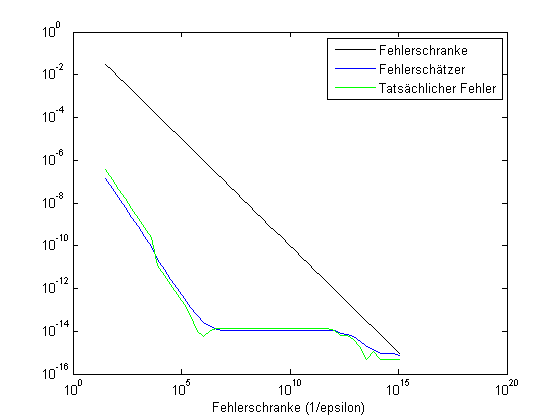
\includegraphics[width = 0.9\textwidth]{sqrtFehler.png}
	\caption{Genauigkeit}
\end{minipage}
\hfill
\begin{minipage}[hbt]{0.4\textwidth}
	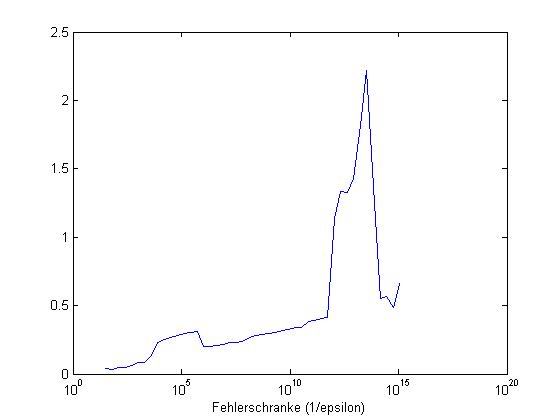
\includegraphics[width = 0.9\textwidth]{sqrtZeit.png}
	\caption{Rechenzeit}
\end{minipage}
\end{figure}

\item $f = @(x) \frac{1}{\sqrt{x}}$, $a = 0$, $b = 1$

\begin{figure}[htbp]
  \centering
\begin{minipage}[hbt]{0.4\textwidth}
	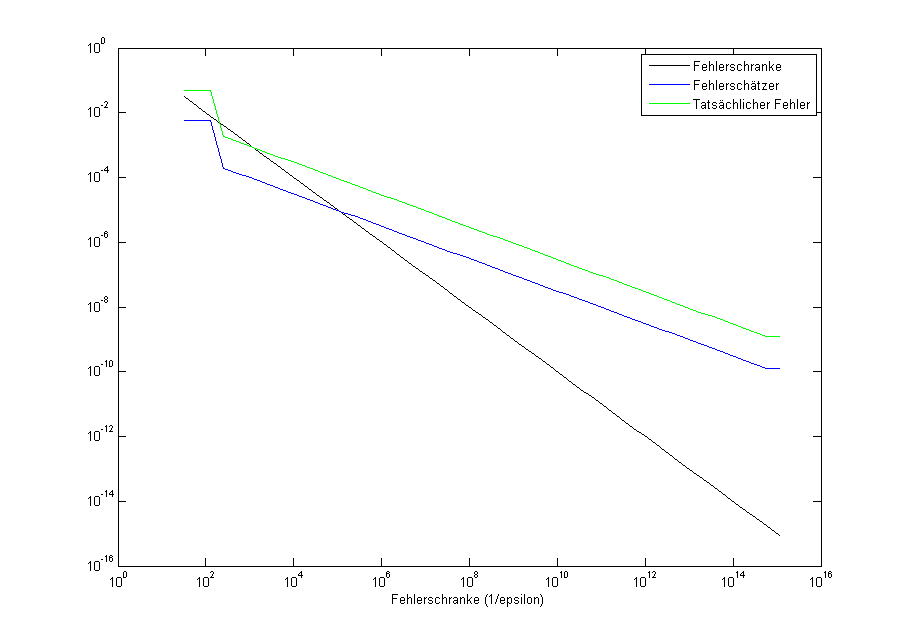
\includegraphics[width = 0.9\textwidth]{1_sqrtFehler.png}
	\caption{Genauigkeit}
\end{minipage}
\hfill
\begin{minipage}[hbt]{0.4\textwidth}
	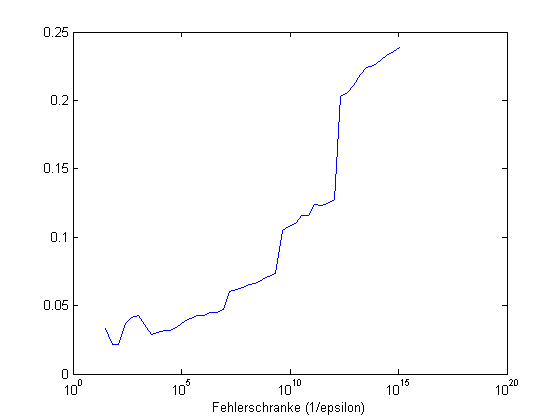
\includegraphics[width = 0.9\textwidth]{1_sqrtZeit.png}
	\caption{Rechenzeit}
\end{minipage}
\end{figure}

\newpage

\item $f = @(x) \sin(x)$, $a = 0$, $b = \pi$
\begin{figure}[htbp]
  \centering
\begin{minipage}[hbt]{0.4\textwidth}
	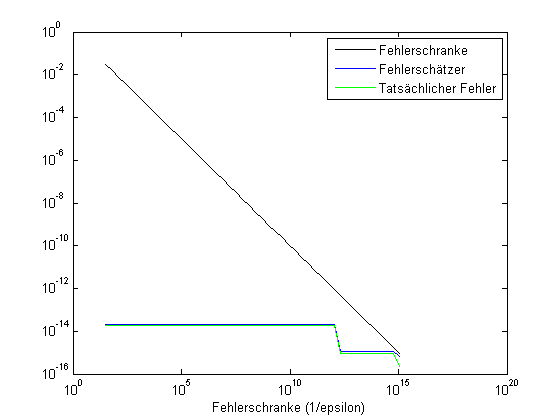
\includegraphics[width = 0.9\textwidth]{sinFehler.png}
	\caption{Genauigkeit}
\end{minipage}
\hfill
\begin{minipage}[hbt]{0.4\textwidth}
	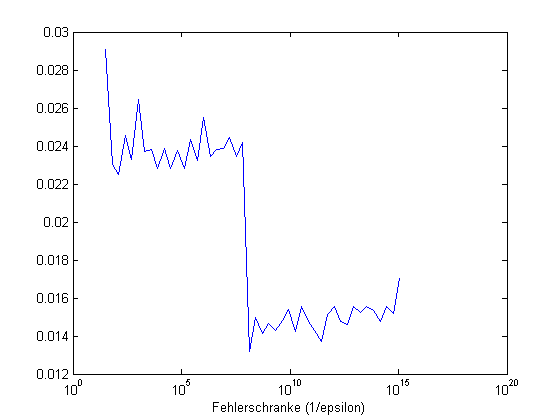
\includegraphics[width = 0.9\textwidth]{sinRechenzeit.png}
	\caption{Rechenzeit}
\end{minipage}
\end{figure}

\item $f = @(x) \sin(\frac{1}{x}) $, $a = 0$, $b = 1$
\begin{figure}[htbp]
  \centering
\begin{minipage}[hbt]{0.4\textwidth}
	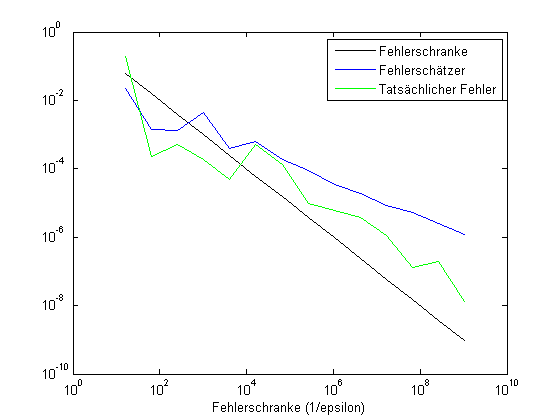
\includegraphics[width = 0.9\textwidth]{sin1_Fehler.png}
	\caption{Genauigkeit}
\end{minipage}
\hfill
\begin{minipage}[hbt]{0.4\textwidth}
	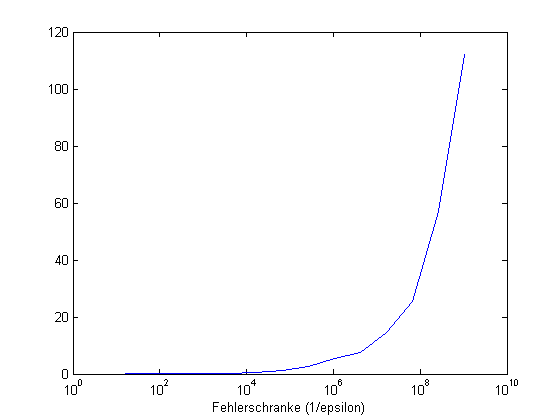
\includegraphics[width = 0.9\textwidth]{sin1_Zeit.png}
	\caption{Rechenzeit}
\end{minipage}
\end{figure}

\end{itemize}

\end{document}


